\documentclass{article}
\usepackage[utf8]{inputenc}
\usepackage{tikz}
\usetikzlibrary{shapes,arrows}
\usepackage[ruled,vlined]{algorithm2e}
%\usepackage{algpseudocode}
\usepackage{multicol}
\renewcommand{\contentsname}{{\Huge Table de Matières}}
\usepackage{titlesec}
\usepackage{xcolor}
\usepackage{listings}
\usepackage{graphicx}
\titleformat{\section}{\huge\bfseries}{\thesection}{1em}{}
\titleformat{\subsection}{\LARGE\bfseries}{\thesubsection}{1em}{}
\titleformat{\subsubsection}{\Large\bfseries}{\thesubsubsection}{1em}{}
\begin{document}
%first page
\begin{center}
\pagenumbering{gobble}
\linespread{2.0}\selectfont

{\Huge U}{\huge NIVERSITÉ DE }{\Huge M}{\huge ONTPELLIER}\\
{\huge L2}{\LARGE ~INFORMATIQUE }
\\~\\~\\~\\~\\
{\Large\textbf{GOLF MATHÉMATIQUE}}
\\~\\~\\~\\~\\

\linespread{1}\selectfont

RAPPORT DE PROJET T.E.R\\
PROJET INFORMATIQUE HLIN405\\
\vfill
\end{center}
\begin{multicols}{2}
\begin{flushleft}
\textbf{Etudiants:}\\
~~M. Mike Germain\\
~~M. Benjamin Baska\\
~~M. Kevin Lastra
\end{flushleft}
\columnbreak
\begin{flushright}
\textbf{Encadrante:}\\
~~Mme. Annie Chateau
\end{flushright}
\end{multicols}
\newpage
%bilan
\pagenumbering{arabic}
\setcounter{page}{1}
\tableofcontents
\newpage
%introduction
{\textbf{\Huge Introduction}}\\~\\~\\
~~Sous la direction de Mme. Annie Chateau, notre groupe, composé de Mike Germain, Benjamin Baska, Kevin Lastra, a travaillé sur le développement du jeu "Golf Mathématique" comme projet du module HLIN405.

\newpage
%cahier de charges
\section{Organisation du projet}
\subsection{Objectifs et cahier des charges}
~\\~\\
Le but est de créer un jeu de golf, version mathématique.
\\~\\
\textbf{\large Base et Règles}
\\~\\
Les règles sont simples:
\\~\\
- Partir du point de départ et aller jusqu'au trou en faisant le moins de coups.
\\~\\
- On ne peut que se déplacer de la portée indiquée sur notre case, dans 8 positions différentes, haut, bas, droite, gauche, ainsi que, haut droite, haut gauche, bas droite, bas gauche (case entouré en noir sur la figure ci-dessous).
\\~\\
\begin{figure}[!h]
\centering
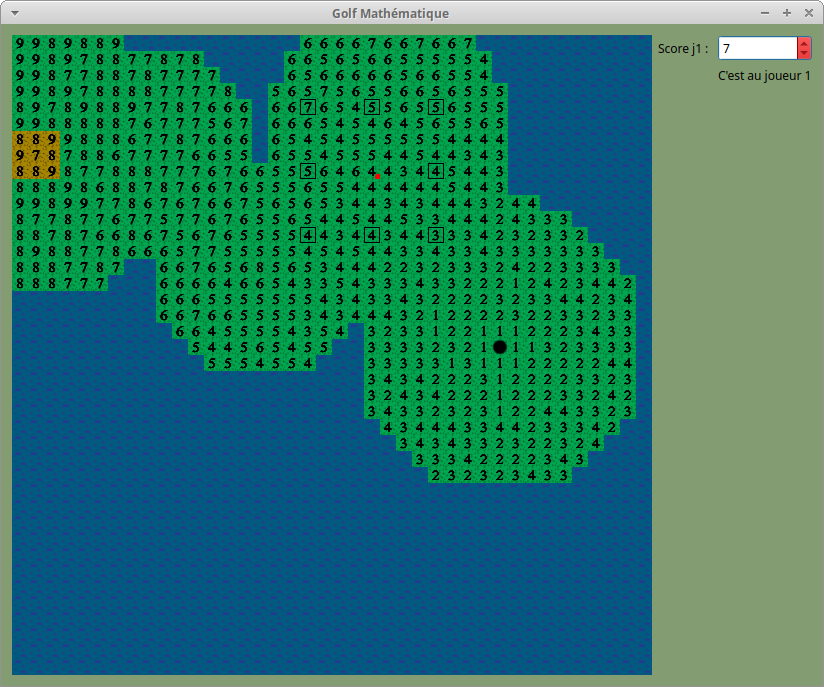
\includegraphics[scale=0.3]{Images/move.png}
\caption{Exemple de déplacement}
\end{figure}
\\~\\
\newpage
\textbf{\large Interface Graphique}
\\~\\
Pour la partie graphique, le but est d'apprendre à utiliser une interface graphique, et rendre plus fluide et convivial le jeu.
\\~\\
\textbf{\large Génération automatique de la carte}
\\~\\
Pouvoir générer des nouveaux terrains pour le jeux et c'était aussi un défi algorithmique.
\\~\\
\textbf{\large Intelligence Artificielle}
\\~\\
Ici, "intelligence artificielle" est compris comme "joueur ordinateur", c'est a dire avoir un adversaire non humain, le travail est donc de créer ce joueur et de déterminer son comportement de manière a rendre le jeu plus intéressant et compétitif.
\\~\\
\newpage
\subsection{Division du travail}
~\\
Nous avons tout d'abord, pris le temps de bien structurer le jeu, ce mettre tous d'accord sur comment on voyait le golf mathématiques.\\
Puis, nous avons séparé le travail en fonction des affinités de chacun, Kevin pour la partie de création d'un algorithme de génération de terrain, Mike pour ce qui est de la création d'une intelligence artificielle et Benjamin pour la partie visuel du jeu et l'adaptation avec la librairie graphique.
\\~\\
\begin{figure}[!h]
\centering
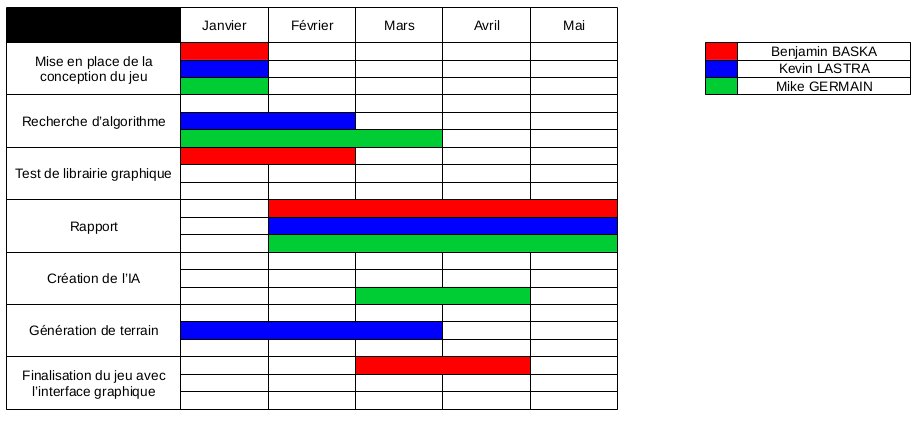
\includegraphics[scale=0.3]{Images/driagram.png}
\caption{Diagramme de Gantt}
\end{figure}
~\\~\\~\\~\\~\\
\tikzstyle{decision} = [diamond, draw, fill=blue!20, 
    text width=4.5em, text badly centered, node distance=3cm, inner sep=0pt]
\tikzstyle{block} = [rectangle, draw, fill=blue!20, 
    text width=5em, text centered, rounded corners, minimum height=4em]
\tikzstyle{line} = [draw, -latex']
\tikzstyle{cloud} = [draw, ellipse,fill=red!20, node distance=3cm,
    minimum height=2em]

\begin{figure}[h]
\centering
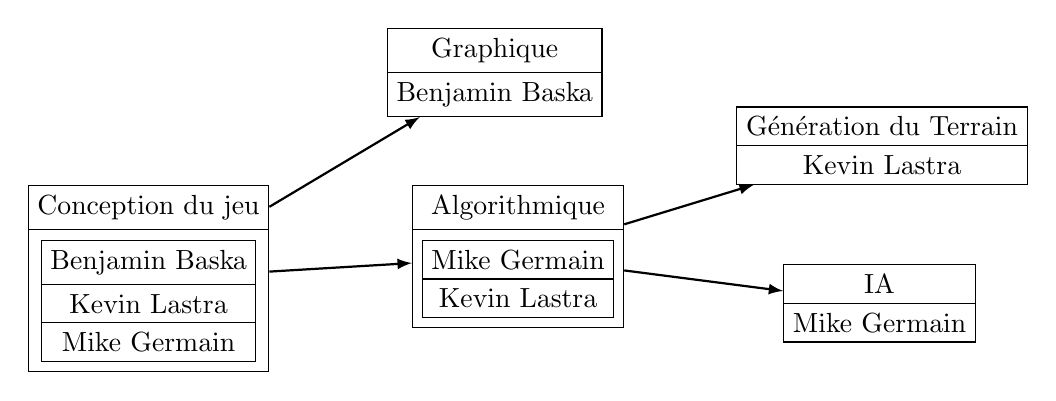
\begin{tikzpicture}[
					double/.style={draw, anchor=text, rectangle split, rectangle split parts=2},
					triple/.style={draw, anchor=text, rectangle split, rectangle split parts=3}]
    % Place nodes
    \node [double] (A) at (-5,0){Conception du jeu
    	\nodepart{second}
    	\tikz{
    		\node[triple]{Benjamin Baska
    		\nodepart{second}Kevin Lastra
    		\nodepart{third}Mike Germain
    		};
    	}
    };
    \node [double] (B) at (0,2){Graphique
    	\nodepart{second}
    	Benjamin Baska
    };
    \node [double] (C) at (0,0){Algorithmique
    	\nodepart{second}
    	\tikz{
    		\node[double]{Mike Germain
    		\nodepart{second}Kevin Lastra
    		};
    	}
    };
	\node [double] (D) at (5.5,-1){IA
    	\nodepart{second}
    	Mike Germain
    };
    \node [double] (E) at (4,1){Génération du Terrain
    	\nodepart{second}
    	Kevin Lastra
    };
    \draw[thick,-latex] (A) edge (B);
    \draw[thick,-latex] (A) edge (C);
    \draw[thick,-latex] (C) edge (D);
    \draw[thick,-latex] (C) edge (E);
    % Draw edges
    
\end{tikzpicture}~\\
\caption{Diagramme de répartition du travail.}

\end{figure}
\newpage
\subsection{Outils de travail}
~\\~\\
\textbf{\large Langage de programmation}\\
Le langage qu'on a choisi pour le développement du jeu, est le C++ pour 2 raisons principales:

\begin{enumerate}
\item Ce langage est un langage de "programmation orienté objets" (POO).
\item Grâce aux modules de HLIN202 et HLIN302, on a une base de connaissance avec laquelle on peut travailler de manière confortable.
\end{enumerate}
~\\~\\
\textbf{\large Outil de modélisation graphique}\\
On a choisi la librairie QT pour les différents avantages qu'elle nous apporte. Cette librairie dispose d'une bonne documentation, elle est adapté au langage C++ et elle dispose aussi d'un outil de travail intéressant appelé "QT Creator", qui rend le travail plus facile.\\~\\~\\
\textbf{\large Travail collaboratif}\\
Nous avons utilisé plusieurs programmes:
\begin{enumerate}
\item GitHub. Ce gestionnaire de version nous permet de partager les avancements du travail réalisé par chacun depuis différents ordinateurs et aussi de sauvegarder plusieurs versions du travail, ce qui est rassurant en cas de perte. 
https://github.com/kevinlastra/GolfMath.git
\item Discord. Celui-ci nous permet le partage d'écran, la communication orale et écrit, ce qui est utile pour le développement du jeu.
\end{enumerate}
~\\~\\
\textbf{\large Éditeur de texte}\\
La production du projet est réalisée grâce à plusieurs éditeur de texte:
\begin{enumerate}
\item Éditeur de code -
Emacs, sublime et QTCreator.
\item Éditeur \LaTeX{} - TexMaker
\end{enumerate} 
\newpage
\section{Conception}
Dès la première réunion, en utilisant l'image qui nous a été donné dans notre sujet de projet, on a cherché une architecture de programmation pour laquelle ce jeu s'adapterait au mieux. Nous avons opté pour une modélisation objet qui permet de bien délimiter chaque élément du jeu.\\
\begin{figure}[!h]
\centering
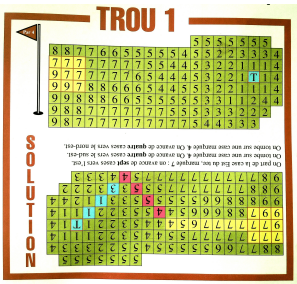
\includegraphics[scale=0.3]{Images/sujet.png}
\caption{Image du sujet}
\end{figure}
\\
La première chose qu'on a défini est la forme du terrain de jeu, Terrain de NxM cases, la forme rectangulaire est la plus adaptée pour gérer le terrain dans l'interface mais le "green" lui-même a sa forme propre à l'intérieur de ce rectangle.  La classe Terrain crée on a structuré une classe qui manipulerait toutes les entrées/sorties ("ToutEnUn") et finalement les joueurs avec une méthode "QEvent".\\
\newpage
% Define block styles
\tikzstyle{decision} = [diamond, draw, fill=blue!20, 
    text width=4.5em, text badly centered, node distance=3cm, inner sep=0pt]
\tikzstyle{block} = [rectangle, draw, fill=blue!20, 
    text width=5em, text centered, rounded corners, minimum height=4em]
\tikzstyle{line} = [draw, -latex']
\tikzstyle{cloud} = [draw, ellipse,fill=red!20, node distance=3cm,
    minimum height=2em]
\begin{figure}[h]
\centering
\begin{tikzpicture}[node distance = 2cm, auto]
    % Place nodes
    \node [block] (OP) {Out Put};
    \node [block, below of=OP] (GM) {ToutEnUn};
    \node [block, right of=GM, yshift=0cm, xshift=2cm] (Ter) {Terrain};
    \node [block, right of=Ter, yshift=0cm, xshift=2cm] (init) {Node};
    \node [cloud, below of=GM] (PC) {QEvent};
    \node [block, below of=init] (IA) {Artificial Intelligence};
    \node [cloud, right of=PC, yshift=-0.5cm, xshift=1cm] (A) {if IA};
    % Draw edges
    \path [line] (init) -- node[near start]{1} node[near end]{[*..,*.]}(Ter);
    \path [line] (Ter) -- (GM);
    \path [line] (GM) -- (Ter);
    \path [line] (GM) -- (OP);
    \path [line] (PC) -- (GM);
    \path [line,dashed] (PC) -- (A);
    \draw [line,dashed] (A) -- (IA);
    \draw [line,dashed] (IA) -- node[above]{send request}(PC);
    \draw [line,dashed] (A) -- node[near start]{else} ++ (-2,0) --++(0,4) -- (OP);
    \draw [line,dashed] (OP) --++ (2.5,-1.2) --++ (0,-2.3) --++ (1,-0.5);
\end{tikzpicture}~\\
\caption{Représentation du flux du jeu.}
\end{figure}
Quand le joueur lance le jeu, il appel la classe "ToutEnUn", qui crée un terrain avec la classe "Terrain", qui celui-ci appel plusieurs case de la classe "Node". Le terrain est ainsi généré.\\
Ensuite quand le joueur clique, il envoie une requête, "send request", à "QEvent", et fait ainsi avancé le jeu, couleur rose du graphique.\\
Si il y a une IA, "if IA", au moment de la requête, l'IA est donc appelé grâce à une méthode, et ainsi retourne à "QEvent" et le jeu continue.
\newpage
\subsection{Base du jeu}
~\\~\\
Golf mathématique est une autre version du golf traditionnel, donc cela signifie qu'on modifie ainsi le jeu sans perdre l'esprit du golf.\\
Le golf est un jeu où plusieurs joueurs jouent tour par tour, la personne gagne si elle a fait le moins de coup, donc le moins de points.\\~\\
Donc pour définir les bases de notre jeu on doit utiliser les règles du jeu original.
Dans un Terrain de golf, on a:
\begin{itemize}
\item Départ (zone où les joueurs commencent)
\item Cible (le trou)
\item Obstacles (zone d'eau)
\end{itemize}
Ici pour des raisons de simplicité nous avons modélisé une seule sorte d'obstacles, mais il serait envisageable d'enrichir le jeu avec différents types (forêt, sable, pierre) qui entraîneraient différents comportements.
\\~\\
Et puis, le joueur se déplace et tape la balle avec une puissance, la portée.\\
Avec tout ça, on a des éléments avec lesquels on peut travailler: un terrain que l'on interprétera comme un tableau d'entiers, les valeurs étant la portée de la balle.\\
Un terrain sera divisé en 4 zones différentes (voir aussi figure 9):
\begin{itemize}
\item Départ, case jaune, c'est sur celle-ci que la partie commence mais elles ont les attributs d'une case herbe.
\item Eau, case bleu, cette case nous fait perdre un tour si on y va dessus et nous renvoie à notre dernière position.
\item Herbe, case verte, elles sont les briques de notre jeu, elles ont chacune une portée.
\item Trou, case avec un rond noir, elle est unique et met fin à la partie.
\end{itemize}
Un dernier type "sable" avait été envisagé pour des cases de faibles portées, mais du au confinement cela a été enlevé.
\newpage
\subsection{Graphique}
~\\
\textbf{\large Choix de la librairie graphique}
~\\
Au début du projet, nous nous avions décidé d'utiliser la librairie graphique SDL\footnote{https://www.libsdl.org/} : 
~\\
\begin{figure}[!h]
\centering

\includegraphics[scale=0.2]{Images/logoSDL.png}
\caption{Librairy SDL.}
\end{figure}
~\\
Mais le fait qu'elle soit adapté au langage C, et donc pas prévu pour de l'orienté objet nous a posé quelque soucis.\\
Après cela, nous avons cherché ainsi une autre librairie, celle ci adapté au C++.\\
Nous nous sommes alors mis d'accord sur Qt \footnote{https://www.qt.io/}. Cette librairie offre une grande documentation et un éditeur de texte adapté ("Qt Creator").
~\\
Les premiers essais pour la partie graphique ont pu commencer, avec en premier les cases de jeu : 
\begin{figure}[!h]
\centering

\includegraphics[scale=1]{Images/green_1.jpg}

\includegraphics[scale=1]{Images/start_1.jpg}
\caption{Première version des dessins}
~\\
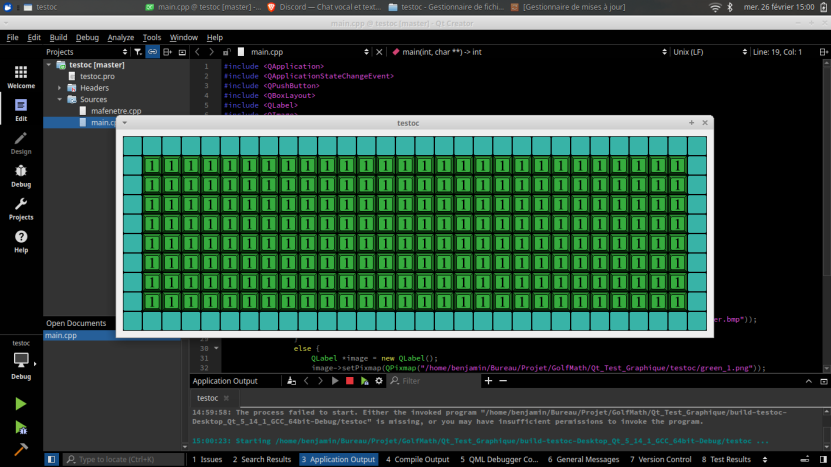
\includegraphics[scale=0.2]{Images/terrain.jpg}
\caption{Premier test de terrain}
\end{figure}
~\\~\\~\\
Le résultat étant trop sombre, on a refait les cases avec un rendu plus clair et plus lisible.\\~\\~\\
\begin{figure}[!h]
\centering

\includegraphics[scale=2]{Images/green.jpg}

\includegraphics[scale=2]{Images/water.jpg}

\includegraphics[scale=2]{Images/hole.jpg}

\includegraphics[scale=2]{Images/start.jpg}
\caption{Rendu deuxième version}
~\\
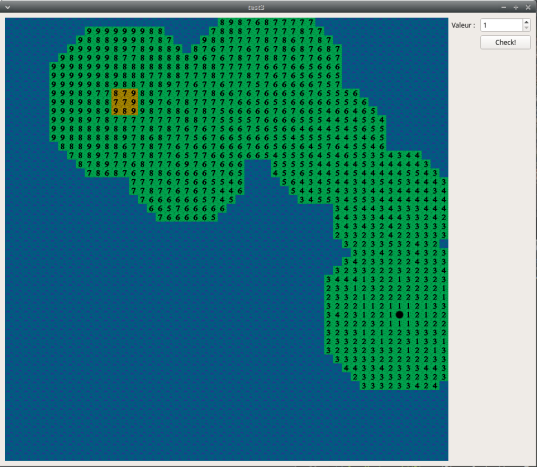
\includegraphics[scale=0.5]{Images/terrain2.jpg}
\caption{Rendu final}
\end{figure}
~\\
\newpage
\subsection{Qt}
~\\~\\
\textbf{\large La création d'une interface}
\\~\\
Pour pouvoir créer une interface graphique, on utilise la librairie et les objets de Qt, tel que QApplication qui permet de gérer l'interface graphique de l'utilisateur (ou GUI en anglais), ainsi que de contrôler le flux d'entrée et de sortie et les paramètres principaux de notre interface.\\
Voilà à quoi ressemble le code principal pour créer une fenêtre :\\
\begin{verbatim}
#include <QApplication>
#include "toutenun.h"
#include "mainwindow.h"

int main(int argc, char *argv[])
{
    QApplication app(argc, argv);

    MainWindow fen;
    fen.show();

    return app.exec();
}
\end{verbatim}
~\\
\begin{verbatim}
QApplication app(argc, argv);
return app.exec();
\end{verbatim}
~\\
C'est cela qui va créer une première fenêtre.\\
Ensuite les autres objets que nous appellerons, hériteront de la classe QObject, une autre classe importante de Qt qui permet l'affichage de widget.\\
\begin{verbatim}
MainWindow fen;
fen.show();
\end{verbatim}
Cela appelle notre classe MainWindow qui est la fenêtre d'accueil de notre jeu.\\~\\
\begin{figure}[!h]
\centering 
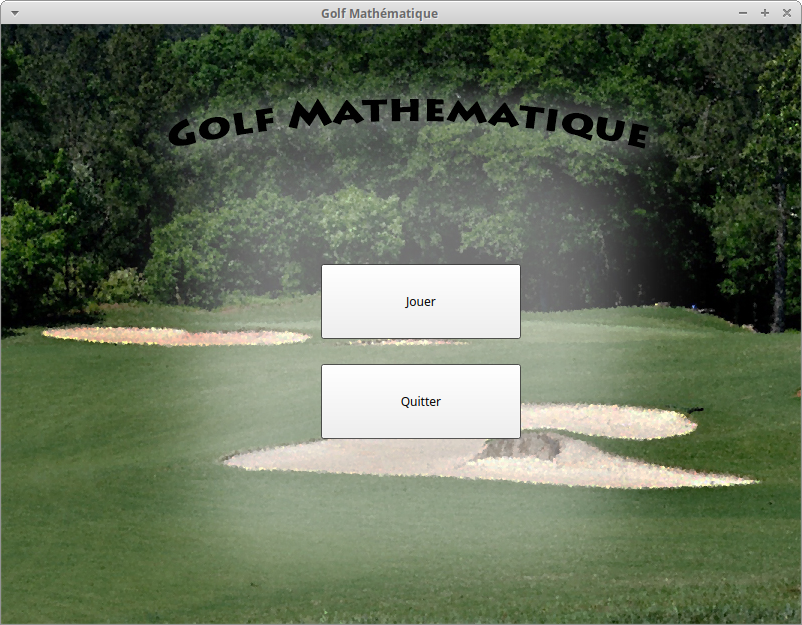
\includegraphics[scale=0.3]{Images/accueil.png}
\caption{Accueil}
\end{figure}
~\\
La classe de cette fenêtre est :
\begin{verbatim}
#include "mainwindow.h"

MainWindow::MainWindow(QWidget *parent) : QMainWindow(parent)
{
    setWindowIcon(QIcon("./image/ballegolf.png"));
    setWindowTitle("Golf Mathématique");
    setFixedSize(800, 600);
    QPalette fond;
    fond.setBrush(backgroundRole(), QBrush(QPixmap("./image/v2/background.jpg")));
    setPalette(fond);

    jouer = new QPushButton("Jouer", this);
    quitter = new QPushButton("Quitter", this);
    jouer->setFixedSize(200, 75);
    quitter->setFixedSize(200, 75);
    jouer->move(320, 240);
    quitter->move(320, 340);

    connect(jouer, SIGNAL(clicked()), this, SLOT(lancer()));
    connect(jouer, SIGNAL(clicked()), this, SLOT(close()));
    connect(quitter, SIGNAL(clicked()), qApp, SLOT(quit()));
}


void MainWindow::lancer()
{
    Niveaux *niv = new Niveaux;
    niv->show();
}
\end{verbatim}
~\\
Ici nous pouvons voir plusieurs nouvelles choses. 
\begin{verbatim}
	setWindowIcon(QIcon("./image/ballegolf.png"));
    setWindowTitle("Golf Mathématique");
    setFixedSize(800, 600);
    QPalette fond;
    fond.setBrush(backgroundRole(), QBrush(QPixmap("./image/v2/background.jpg")));
    setPalette(fond);
\end{verbatim}
Toute cette partie s'occupe de l'apparence de la fenêtre, son nom et son icône.
\begin{verbatim}
    jouer = new QPushButton("Jouer", this);
    quitter = new QPushButton("Quitter", this);
    jouer->setFixedSize(200, 75);
    quitter->setFixedSize(200, 75);
    jouer->move(320, 240);
    quitter->move(320, 340);
\end{verbatim}
Celle ci s'occupe des widgets comme les boutons.
\begin{verbatim}
    connect(jouer, SIGNAL(clicked()), this, SLOT(lancer()));
    connect(jouer, SIGNAL(clicked()), this, SLOT(close()));
    connect(quitter, SIGNAL(clicked()), qApp, SLOT(quit()));
\end{verbatim}
Ensuite, on attribut un effet à nos boutons.
\begin{verbatim}
void MainWindow::lancer()
{
    Niveaux *niv = new Niveaux;
    niv->show();
}
\end{verbatim}
Et enfin, cette méthode appelle notre nouvelle fenêtre qui gère nos différents niveaux (figure 12).\\
\begin{figure}
\centering
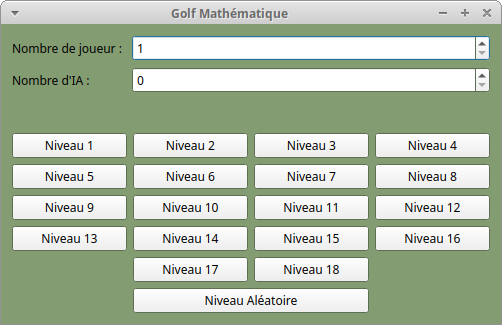
\includegraphics[scale=0.5]{Images/niveaux.png}
\caption{Page des niveaux}
\end{figure}
Les niveaux lancent alors différentes seeds (référence des niveaux), ces seeds servent à générer à la volée de nouveaux terrains (figure 13).\\
\begin{figure}
\centering
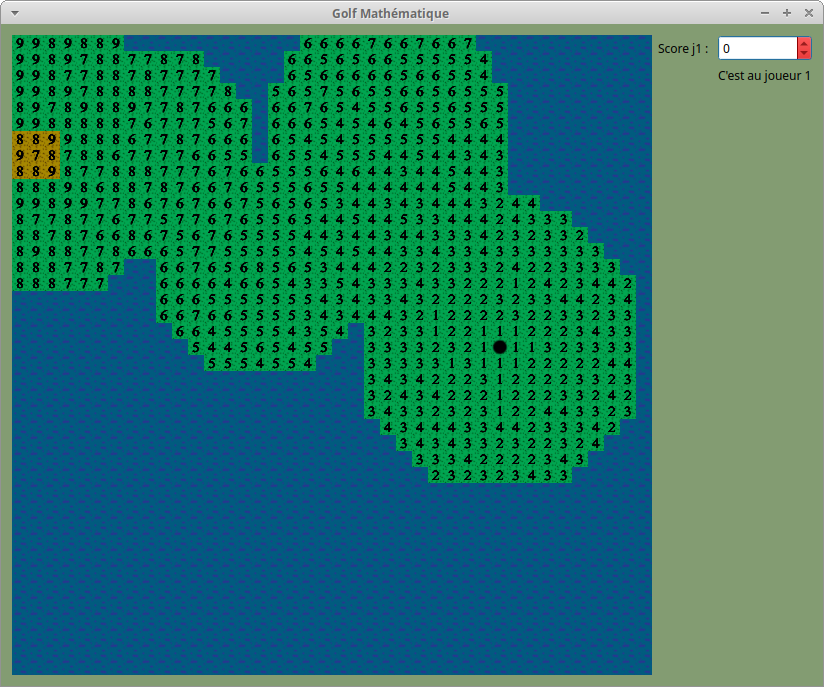
\includegraphics[scale=0.3]{Images/niveau1.png}
\caption{Niveau 1}
\end{figure}
\newpage
\subsection{Intelligence Artificielle - IA}
\subsubsection{Une IA pas très futée}
La première idée pour faire l'IA était de faire une basique qui avance tout droit vers le trou sans réfléchir. Son objectif a chaque coup calculer simplement le coup qui se rapprochait le plus du trou avec une boucle 'for' très simple.\\
Un problème en est ressorti, c'est peu efficace dans le sens où le nombre de coups était très élevé par rapport à ce que pouvaient faire les joueurs humains. Cela manque d'intérêt et il vaut mieux jouer contre un adversaire un peu plus fort. Nous avons donc décidé de reprendre du début.\\
\subsubsection{Une IA un peu plus complexe}
Après avoir recherché des algorithmes de recherche de chemins optimaux (pathfinding) sur internet, un algorithme en particulier en est ressorti assez souvent : A* (ou A star)\\
C'est un algorithme de pathfinding très connu qui ressemble à ceci :
\begin{verbatim}
Fonction cheminPlusCourt(g:Graphe, objectif:Nœud, depart:Nœud)
       closedList = File()
       openList = FilePrioritaire(comparateur=compare2Noeuds)
       openList.ajouter(depart)
       tant que openList n'est pas vide
           u = openList.depiler()
           si u.x == objectif.x et u.y == objectif.y
               reconstituerChemin(u)
               terminer le programme
           pour chaque voisin v de u dans g
               si non(v existe dans closedList ou si v existe
                dans openList avec un cout inférieur)
                    v.cout = u.cout +1 
                    v.heuristique = v.cout + distance([v.x, v.y], 
                    [objectif.x, objectif.y])
                    openList.ajouter(v)
           closedList.ajouter(u)
       terminer le programme (avec erreur)
\end{verbatim}
L'idée de cet algorithme est d'améliorer un chemin déjà trouvé en regardant les chemins voisins et ce jusqu'à ne plus pouvoir l'améliorer. Nous avons ensuite du évidemment adapter l'algorithme à notre projet, pour se faire nous avons d'abord du créer une classe qui à une case associe un 'coût' (le nombre de coups jusqu'ici), une heuristique (la distance "à vol d'oiseau" jusqu'à l'arrivée ce qui permet de minorer la distance réelle à parcourir) et un père, pour à la fois pouvoir recréer le chemin après le pathfinding mais aussi tout simplement pour le bon fonctionnement de l'algorithme. \\~\\
Et après plusieurs complications, cette IA était enfin terminée et fonctionnelle. A savoir que, bien que l'IA trouve le meilleur chemin à chaque fois, elle n'est pas invincible, il n'est pas compliqué de faire égalité ou même de la battre car nous avons fait en sorte qu'elle ne choisisse pas son point de départ de manière optimale.
\newpage
\subsection{Génération du Terrain}
\subsubsection{Génération Automatique}
Pour générer un terrain de manière automatique on doit placer des règles:
\begin{itemize}
\item Le Terrain doit être connexe ou au moins cheminable.
\item La génération des portées doit être presque linéaire.

\end{itemize}
Après avoir testé différentes idées, nous avons trouvé une solution très convenable pour construire un terrain. Pour générer notre terrain on va produire un chemin autour duquel on va faire apparaître la surface jouable.\\
Cette algorithme est divisé en deux passages sur une grille :\\~\\
\textbf{\Large{Premier Passage}}\\
On produit un premier point de manière aléatoire $P_0$ = (x, y), et à partir de ce point on génère n-1 autres points ($P_0$,...,$P_n$).
\begin{center}
	$P_{k} = P_{k-1} + B_k(a, b)$
\end{center}
Telle que $k\leq$ n, $k>0$, le vecteur (a , b) $\in$ V valide (V l'ensemble des 8 différentes directions valides représenté avec des vecteurs).
\begin{center}
	V = \{(-1,-1),(-1,0),...,(1,1)\}
\end{center}	
Un vecteur (a , b) est valide uniquement si la distance entre $P_0$ et $P_{k-1}$ est inférieur a la distance entre $P_0$ et $P_k$.\\
B est un tableau d'entier arbitrairement sélectionnée, par exemple :
\begin{center}
	B = \{8,8,7,6,5,4,3,2,2\}\\
\end{center}
dans ce cas B est un tableau de 9 entier avec les extrémités doubles, pour augmente la vitesse du jeux au début et éviter le nombre 0 a la fin, a cause du deuxième passage.
\begin{center}
	$B_n = B_{n-1}$ et $B_0 = B_1$.
\end{center}

Avec cet algorithme on trouverait que:\\~\\
X:"l'ensemble des terrains générés" \\
Y:"l'ensemble des chemins possibles"\\
\(\forall x \in X, \exists y \in Y\) telle que "y" est un chemin valide.\\~\\
On définit un chemin valide, le chemin connexe et jouable dans 15 ou moins mouvement.\\
Avec cette phrase on peut générer le terrain sans avoir à penser aux possibles contraintes comme la connexité.
\newpage
\textbf{\Large{Pseudo Code}}\\~\\
\begin{algorithm}[H]
	\caption{GénérationChemin(d lo: entier, d la: entier,d n: entier): Tableau d'entier}
	\SetKwInOut{Parameter}{variables}
	\SetKwInOut{Debut}{début algorithme}
	\SetKwData{I}{i}\SetKwData{LO}{lo}\SetKwData{LA}{la}
	\SetKwData{DIR}{dir}\SetKwData{Va}{v.x}\SetKwData{Vb}{v.y}
	\SetKwData{V}{v}
	\SetKwArray{TAB}{Tab}\SetKwData{N}{n}
	\SetKwFunction{Random}{random}\SetKwFunction{GDIR}{getdirection}
	\SetKwFunction{NPOS}{nouvellePosition}	
	\Parameter{Tab: tableau d'entier bidimensionnel de taille n*m.\\
	i: entier.\\
	v: structure vecteur contenant une paire d'entier\\ "x" et "y".}
	\Debut\\
	\BlankLine
	\I $\leftarrow 1$\;
	\tcp{on définit v le premier point du chemin.}
	\Va $\leftarrow$ \Random{}$\%$($\frac{lo}{2}$)\;
	\Vb $\leftarrow$ \Random{}$\%$($\frac{la}{2}$)\;
	\TAB{\Va}$[$\Vb$]$ $\leftarrow$ 1\;
	\While{\I $<$ \N}
	{
		\DIR $\leftarrow$ \GDIR{}\;\tcp{renvoie un nombre entre {0-7} aléatoirement, qui représente les 8 différentes directions}
		\V $\leftarrow$ \NPOS{\V ,\DIR}\;\tcp{renvoie un vecteur qui représente la nouvelle position $v_{n+1}$ par rapport à la direction et la position $v_{n}$;}
		\If{\V est valide $\&\&$ \TAB{\Va}$[$\Vb$]$ $==$ 0}
		{
			\TAB{\Va}$[$\Vb$]$ $\leftarrow 1$\;
		}
	}
	\Return \TAB\;
\end{algorithm}
~\\~\\
\newpage
Cet algorithme va nous renvoyer un tableau d'entiers, que l'on peut représenter avec un graphe :\\
GénérationTerrain(n,m,5);\\
\begin{figure}[h]
\centering
\begin{tikzpicture}
%nodes
\node [draw, rectangle,label = "Terrain"
		,minimum size = 3cm] (map) 
{
\begin{tikzpicture}
	\foreach \point [count=\i] in {(-5,4),(-4,5.2),(-3,4),(-2,2.5),(-3,1)}
	{
	\fill \point circle (2pt);
	\draw[black, thick] \point circle (1cm);
	\draw[red] \point+(0,0.5) node {$\i$};
	}
\end{tikzpicture}
};
\end{tikzpicture}~\\
\caption{les cercles représentent la zone ou le Terrain va se générer.}
\end{figure}\\~\\~\\
\definecolor{color1}{RGB}{166,65,180}
\definecolor{color2}{RGB}{55,91,3}
\textbf{\Large{Deuxième Passage}}\\
Le chemin ainsi généré, on va passer case par case dans notre grille et on va tester si la distance entre la case et un point du chemin est inférieure à un certain nombre.
On pose (x, y) une case, T l'ensemble des points du chemin, $\lambda$ le rayon.
\begin{center}
Si distance((x, y), $T_i$) $< \lambda$ alors la case est valide.
\end{center}
Si une case est valide ça veut dire que cette case fait partie de la surface de notre terrain, donc on doit lui donner une portée, cette portée est définie par la formule suivante:
\begin{center}
	portée = {\color{color1}$(2 + (\frac{dist*8}{sranyon}\%8))$} + 
	{\color{color2}$(((rand()\%5)-2)\%2)$}
\end{center}
Cette formule est divisée en 2 parties, représentées par les couleurs:
\begin{center}
	1.~~~~~ $(2 + (\frac{dist*8}{sranyon}\%8))$
\end{center}
\textbf{dist} est la distance entre le dernier point du chemin et la case actuelle.\\
\textbf{srayon} est la distance entre le dernier point du chemin et le point valide le plus éloigné du dernier point du chemin.\\
A l'aide de GeoGebra on peut représenter cette formule de manière plus graphique.\\
\begin{figure}[!h]
\centering
 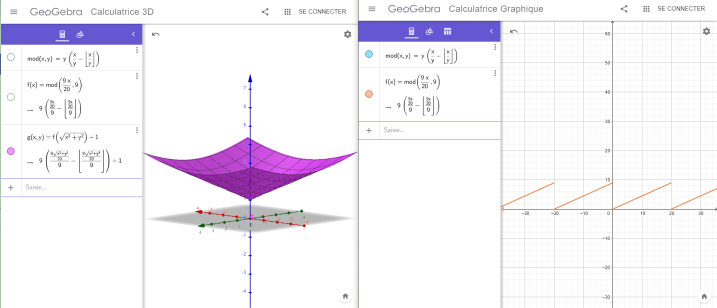
\includegraphics[scale=0.5]{Images/Geogebraimg1.png}\\
 \caption{srayon $=$ 20, 9 au lieu 8 et 1 au lieu 2. La portée d'un point est représentée sur l'axe z.}
\end{figure} 
\begin{center}
	2.~~~~~ $(((rand()\%5)-2)\%2)$\\
\end{center}
rand() un nombre aléatoire entre 0 et RAND{\_}MAX(un nombre très grand qui dépend du langage);
\begin{center}
 $rand()\%5 \leftarrow$ est un nombre entre 0 et 4\\
 $((rand()\%5)-2) \in\{-2,-1,0,1,2\}$\\~\\
 3 nombre pair(60$\%$) et 2 nombre impair(40$\%$).\\~\\
 $(((rand()\%5)-2)\%2) \in\{-1,0,1\}$,\\~\\
\end{center}
ça veut dire qui est plus probable d'avoir 0 que 1 ou -1 donc 60$\%$ de probabilité de ne pas modifier et 40$\%$ pour modifier.

\begin{center}
\newpage
\textbf{\Large{Pseudo Code}}
\end{center}
\begin{algorithm}[H]
	\caption{GénérationTerrain(d Tab: tableau d'entier,d Ch:tableau de vecteur(les points du chemin),d lo:entier,d la:entier): Tableau d'entier}
	\SetKwInOut{Parameter}{variables}
	\SetKwInOut{Debut}{début algorithme}
	\SetKwData{X}{x}\SetKwData{LO}{lo}\SetKwData{LA}{la}
	\SetKwData{Y}{y}\SetKwArray{CH}{Ch}\SetKwData{EXT}{ext}
	\SetKwArray{TAB}{Tab}
	\SetKwFunction{Random}{random}\SetKwFunction{INRAD}{dansRayon}
	\SetKwFunction{FEXTREM}{extrem}	\SetKwFunction{PORTEE}{calcPortee}	
	\Parameter{}
	\Debut\\
	\BlankLine
	\EXT $\leftarrow$ \FEXTREM{\TAB}\;
	\tcp{renvoie le point le plus éloigné du dernier point du chemin(Ch[n-1]).}
	\For{$\X \leftarrow 0$ \KwTo \LO}
	{
		\For{$\Y \leftarrow 0$ \KwTo \LA}
		{
		\BlankLine
			\If{\INRAD{\TAB{\X}$[$\Y$]$,\CH} et \TAB{\X}$[$\Y$]$ $\notin$ \CH}
			{
				\tcp{dansRayon renvoie vrai ou faux dépendamment si un point (x, y) est dans le rayon d'un point du chemin.}
				\TAB{\X}$[$\Y$]$ $\leftarrow$ \PORTEE{\EXT ,\CH{n-1},\TAB{\X}$[$\Y$]$}\;
				\tcp{calcPortee renvoie la portée d'un point utilisant la formule vue avant.}
			}
		}
	}
	\Return \TAB\;
\end{algorithm}
\begin{figure}[!h]
	\centering
	\begin{tikzpicture}
		%nodes
		\node [draw, rectangle,label = "Terrain"
			,minimum size = 3cm] (map) 
			{\begin{tikzpicture}
				\foreach \point [count=\i] in {(-5,4),(-4,5.2),(-3,4),(-2,2.5),(-3,1)}
				{\draw[black, fill] \point circle (1.5cm);}
			\end{tikzpicture}};
	\end{tikzpicture}
	\caption{les zones noires représentent la surface jouable.}
\end{figure}
\newpage
\section{Résultat}
\subsection{Le jeu}
Le jeu est terminé, il est possible de jouer dans 3 mode, tout seul pour s'entraîner, avec d'autre personne jusqu'à 4 joueurs, ou alors avec une IA.\\
Le joueur humain choisit son niveau entre 18 niveaux qui forment un parcours sans monter en difficulté, et un bouton de génération de niveau aléatoire.\\~\\
Le jeu se déroule en cliquant sur le terrain, comme montrer sur la figure 1, chaque joueur à une couleur définie. Rouge pour le joueur 1, bleu pour le joueur 2, jaune pour le joueur 3 et enfin vert pour le joueur 4.
\begin{figure}[!h]
\centering
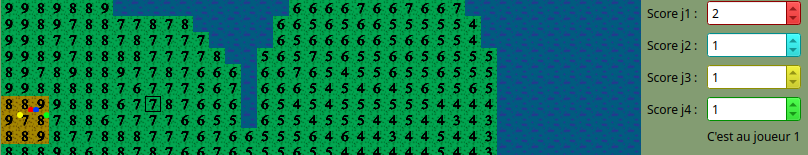
\includegraphics[scale=0.3]{Images/joueur.png}
\caption{Les différents joueurs}
\end{figure}
\\
Quand on ajoute une IA, on ne peut jouer que jusqu'à trois joueurs et l'IA prend la place du dernier joueur.
\subsection{CONCLUSION}
Pour ce qui est de la programmation, nous avons pu mettre en œuvre dans un projet concret ce que l'on a appris en cours. Nous avons amélioré nos compétences techniques personnelles mais aussi notre capacités à s'adapter dans un projet de groupe.\\
Nous avons appris à gérer un projet en équipe avec les atouts de chacun, et aussi apprendre à combler les lacunes que chacun pouvaient avoir.\\~\\
Cependant, en ce qui concerne le projet, nous pouvons imaginer comme amélioration de rajouter plusieurs niveaux d'IA, mettre une difficulté croissante pour les niveaux, on pourrait aussi rajouter de la diversité dans les obstacles du jeu comme des bancs de sable ou encore des arbres. En ce qui concerne l'interface, on pourrait y ajouter des "animations" pour les mouvements de la balles. Le dernier ajout pour rendre le jeu plus optimal serait d'ajouter une partie réseaux.
\newpage
\section{Bibliographie}
En general:
\begin{itemize}
\item www.cplusplus.com/reference
\end{itemize}
Pour la partie graphique on a utilisé les sites suivants :
\begin{itemize}
\item wiki.libsdl.org/FrontPage
\item openclassrooms.com/fr/courses/19980-apprenez-a-programmer-en-c/17117-installation-de-la-sdl
\item doc.qt.io/
\item openclassrooms.com/fr/courses/1894236-programmez-avec-le-langage-c/1898935-initiez-vous-a-qt
\item www.youtube.com/channel/UC6CdzK3QAxtr7giBwqk5eUA
\end{itemize}

\end{document}
